\documentclass{article}
\setlength{\parindent}{0pt}
\usepackage[spanish]{babel}
\usepackage{colortbl}
\usepackage{graphicx}
\usepackage{listings}
\usepackage{hyperref}
\usepackage{minted}
\setminted{%
  breaklines=true,
  autogobble=true,
  bgcolor=yellow,
  fontsize=\footnotesize,
  frame=lines,
  framesep=2mm,
  baselinestretch=1.2,
  linenos
}
\newminted{bash}{%
    linenos,
    autogobble,
    frame=lines,
    framesep=2mm,
    baselinestretch=1.2,
    fontsize=\footnotesize,
    mathescape,
    breaklines % <-- Agrega esta opción
}
% Definir el entorno para el código de shell
\lstnewenvironment{shell}{%
  \lstset{%
    language=bash,
    basicstyle=\ttfamily,
    breaklines=true,
    columns=fullflexible
  }
}{}
% Set page size and margins
\usepackage[letterpaper,top=2cm,bottom=2cm,left=3cm,right=3cm,marginparwidth=1.75cm]{geometry}

\begin{document}

\thispagestyle{empty}
\begin{titlepage}
\centering
\begin{center}
\begin{tabular}{c c}

\includegraphics[width=0.25\textwidth]{gg.png}\hspace{5cm}&\hspace{6cm}
\includegraphics[width=0.25\textwidth]{download.png}\\
\end{tabular}
\end{center}

{\scshape\LARGE Universidad Nacional Autónoma de México \par}
\vspace{2cm}
{\scshape\Large Programa de Tecnología y Cómputo \par}
\vspace{2cm}
{\Large GUÍA DE INSTALACIÓN DE MATLAB EN GNU/LINUX UBUNTU\par}
\vfill
\begin{figure}[ht]
\centering

\includegraphics[width=.5\textwidth]{uno.png}
\end{figure}
{\Large Dulce Michelle Barrios Aguilar \par}

\vfill
{\Large Generación 45º\par}
\vfill
{\Large 18 de noviembre, 2023 \par}
\end{titlepage}
%=======================================================================================
\newpage
\color{black}
\tableofcontents
\newpage 
\section*{Introducción}
\addcontentsline{toc}{section}{Introducción}

MATLAB es una plataforma integral para programación y cálculo numérico, ampliamente adoptada por millones de ingenieros y científicos. Su utilidad radica en la capacidad para analizar datos, elaborar algoritmos y construir modelos de manera eficiente. Lo distintivo de MATLAB radica en su entorno de escritorio optimizado para el análisis iterativo y el diseño, que se combina de manera fluida con un lenguaje de programación diseñado para expresar directamente conceptos matemáticos relacionados con matrices y arrays. Esta integración eficaz facilita a los usuarios llevar a cabo tareas complejas de manera más intuitiva y productiva.\\

La instalación de este software en un sistema operativo basado en GNU/Linux como Ubuntu, implica seguir algunos pasos específicos, los cuales, serán mostrados a continuación.\\
\section*{Paso 1}
\addcontentsline{toc}{section}{Paso 1}
Dirigirse a la URL \href{https://matlab.mathworks.com/}{Matworks} e iniciar sesión.

\begin{figure}[ht]
\centering
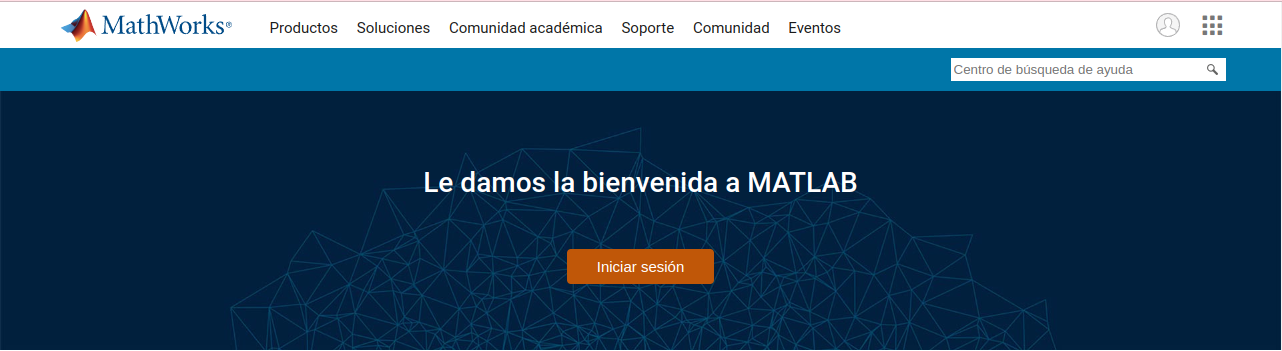
\includegraphics[width=1\textwidth]{dos.png}
\end{figure}
\section*{Paso 2}
\addcontentsline{toc}{section}{Paso 2}
Una vez ingresado, dirigirse a la pestañana "Instalar MATLAB".\\
\begin{figure}[ht]
\centering
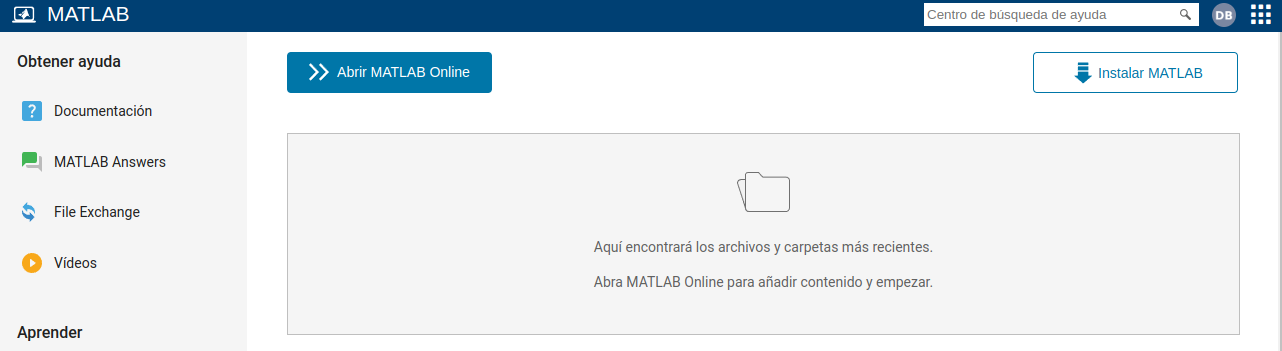
\includegraphics[width=1\textwidth]{tres.png}
\end{figure}
\newpage
Al dar click en el apartado antes mencionado, se mostrará una ventana de Descargas en las que se detecta automáticamente el sistema operativo en el que estamos trabajando, en este caso Linux. Dejar las opciones mostradas por default y dar click en "Descargar para Linux" 
\begin{figure}
\centering
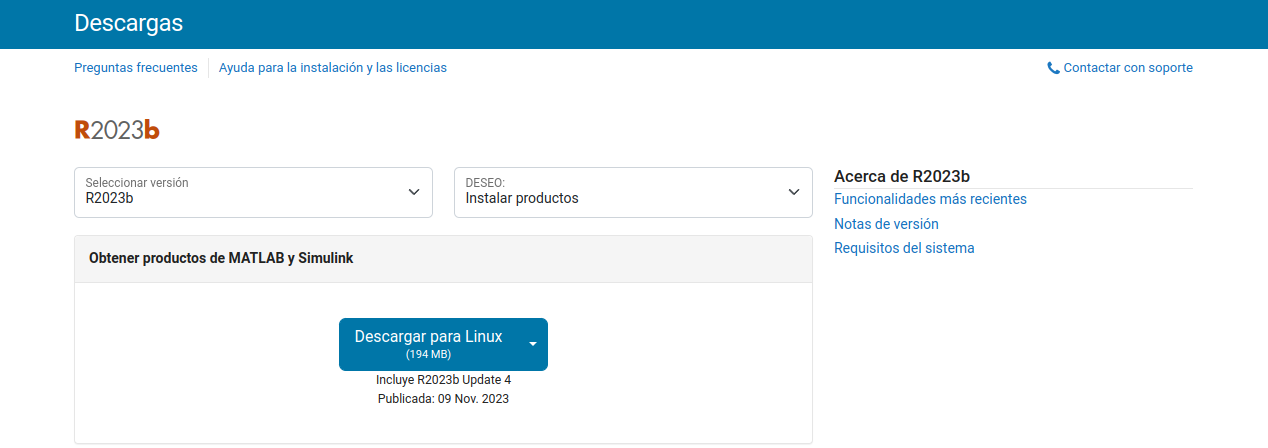
\includegraphics[width=1\linewidth]{image.png}
\end{figure}
\section*{Paso 3}
\addcontentsline{toc}{section}{Paso 3}
Se descargará un archivo comprimido que contiene el instalador de MATLAB. Descomprime el instalador de MATLAB Runtime en la terminal utilizando el comando unzip.\\

Por ejemplo, si estás descomprimiendo el instalador de MATLAB Runtime R2023b, en la terminal, escribe:
\begin{verbatim}
unzip MATLAB_Runtime_R2023b_glnxa64.zip
\end{verbatim}
\section*{Paso 4}
\addcontentsline{toc}{section}{Paso 4}
Dirigirse a la carpeta Descomprimida y ejecutar el siguiente comando:
\begin{verbatim}
sudo -H ./install
\end{verbatim}

Al ser una instrucción con permisos de superusuario se pedirá la contraseña y a continuación se abrirá una ventana como se muestra en la imagen. 

\begin{figure}[ht]
\centering
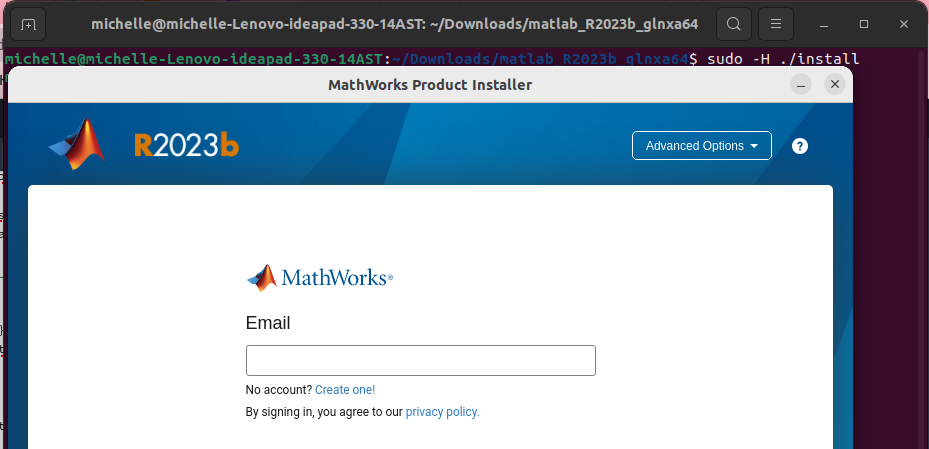
\includegraphics[width=1\textwidth]{cuatro.png}
\end{figure}
\newpage
\section*{Paso 5}
\addcontentsline{toc}{section}{Paso 5}
En la ventana que se abrió, ingresar las credenciales necesarias.\\

Seguidamente, aceptar los términos y condiciones y seleccionar la licencia a instalar. \\
\begin{figure}[ht]
\centering
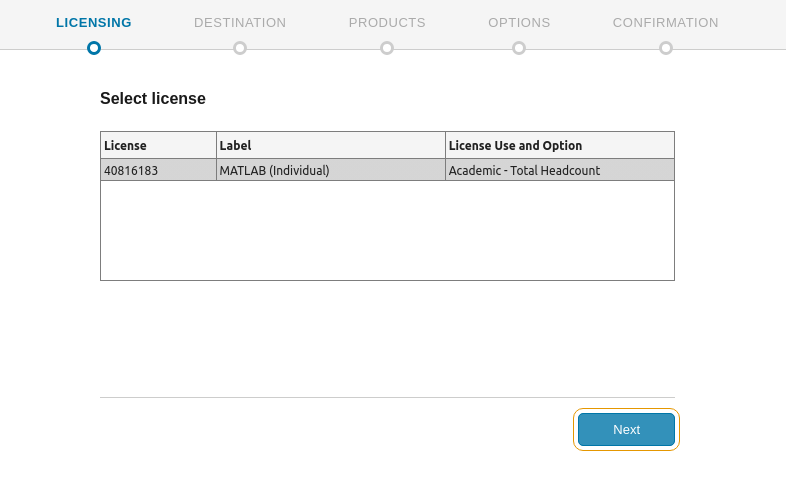
\includegraphics[width=1\textwidth]{cinco.png}
\end{figure}
\section*{Paso 6}
\addcontentsline{toc}{section}{Paso 6}
Elegir la ruta en donde se encontrará MATLAB, así como el producto. MATLAB nos ofrece distintas funcionalidades sin embargo, se recomienda solo instalar las opciones recomendadas. 
\begin{figure}[ht]
\centering
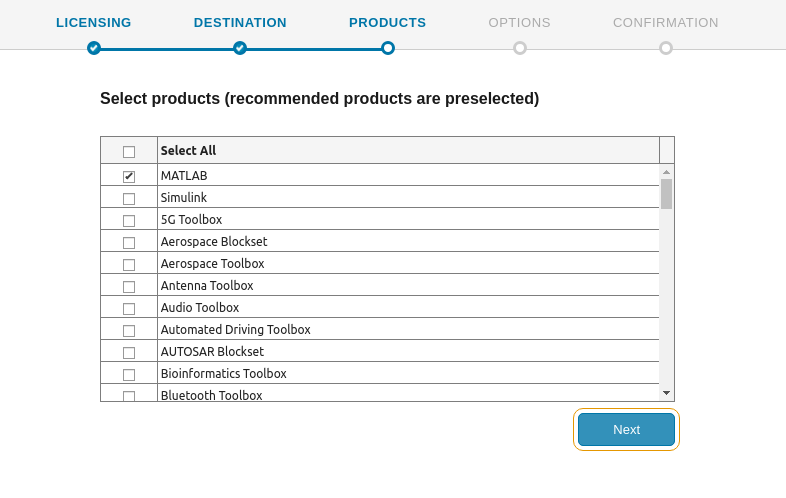
\includegraphics[width=0.7\textwidth]{six.png}
\end{figure}
\section*{Paso 7}
\addcontentsline{toc}{section}{Paso 7}

La instalación comenzará como en la siguiente imagen.

\begin{figure}[ht]
\centering
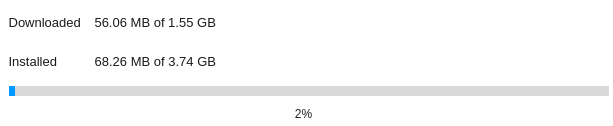
\includegraphics[width=1\textwidth]{ocho.png}
\end{figure}
\section*{Paso 8}
\addcontentsline{toc}{section}{Paso 8}
Y listo! Tu instalación ha sido completada con éxito
\begin{figure}[ht]
\centering
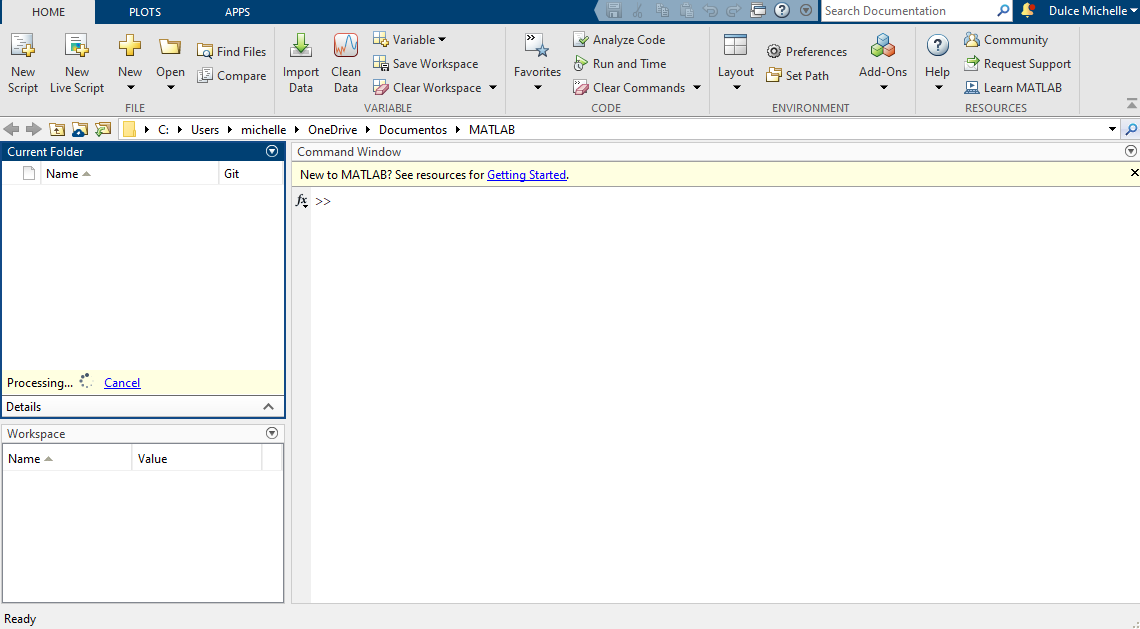
\includegraphics[width=1\textwidth]{nueve.png}
\end{figure}
\end{document}
